\section{Analyse}

\TODO{erledigen}

\subsection{Rundenfunktion}

\begin{figure}[ht]
  \centering
  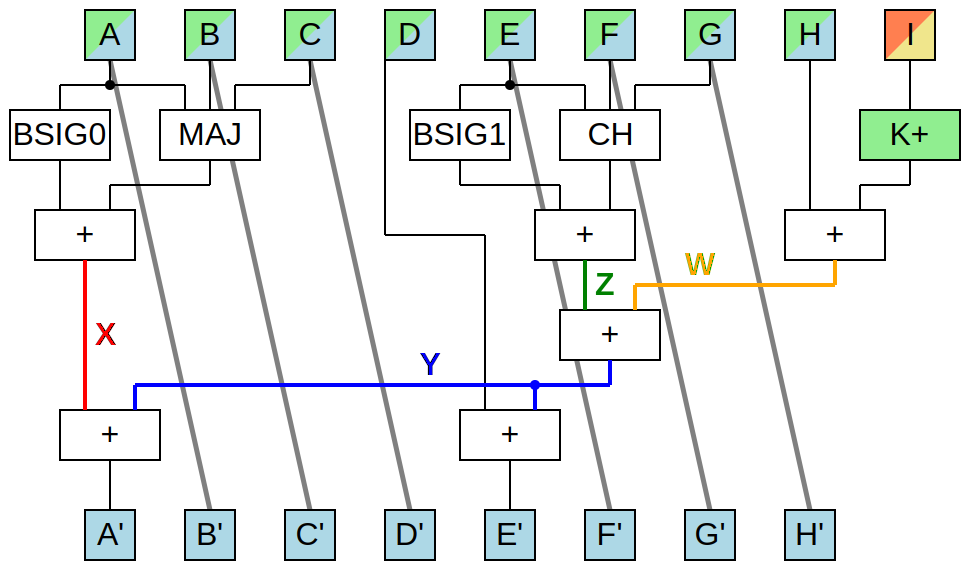
\includegraphics[scale=0.4]{images/sha256coreA}
  \caption{Analyse einer SHA256-Runde}
  \label{fig:sha256coreA}
\end{figure}

D = E' + \textcolor{red}{\textbf{X}} - A'

\subsection{Angriffsvectoren}

A bis H bei gegebenem Hash und Eingabe berechnen.\\
I jeweils bekannt jedoch fehlt A' bis H' da durch Addition mit Geheimnis "`maskiert"'.\\
Würde einen Angriff auf das Lösen einer einmalige Anwendung der 64 Runden bei beliebigen Eingabelängen reduzieren.
~\\
Eingabe bei gegebenem A bis H und Hash berechnen.\\
Problem ist es H/I zu bestimmen wie im Abschnitt vorher beschrieben